\documentclass[a5paper,DIV=12,BCOR=9mm,headsepline,headings=small,cleardoubleempty,10pt]{scrbook}
\usepackage{scrpage2}
\usepackage[colorinlistoftodos, textsize=tiny]{todonotes}
\usepackage{20yearsofKDE}
\usepackage[utf8]{inputenc}
\usepackage{textcomp}
\usepackage{graphicx}
\usepackage{xcolor}
\usepackage{tabularx}
\usepackage[english]{babel}
\usepackage[raiselinks=true,
bookmarks=true,
bookmarksopenlevel=1,
bookmarksopen=true,
bookmarksnumbered=true,
hyperindex=true,
plainpages=false,
pdfpagelabels=true,
pdfborder={0 0 0.5}
]{hyperref}

% Meta data
\newcommand{\booktitle}{20 Years of KDE}
\newcommand{\booksubtitle}{Past, Present and Future}
\newcommand{\bookeditor}{Lydia Pintscher}
\newcommand{\bookyear}{2016}
\newcommand{\bookisbn}{TODO\todo{add ISBN}}
\newcommand{\bookurl}{http://TODO.org\todo{add url}}
\newcommand{\bookauthors}{Lydia Pintscher, TODO\todo{add other authors}}

\hypersetup{
  pdfauthor={\bookauthors},
  pdftitle={\booktitle},
  pdfsubject={Open Source, Free Software, KDE},
  pdfkeywords={Open Source, Free Software, KDE},
  pdflang=en,
  colorlinks,
  linkcolor=black,
  anchorcolor=black,
  filecolor=black,
  urlcolor=black,
  citecolor=black,
  bookmarksnumbered=true,
  pdfpagelayout=TwoColumnRight
}
\ifusinght
\else
  \usepackage{xmpincl}
  \includexmp{20yearsofKDE}
  \usepackage{pdfpages}
\fi
\hyphenation{pro-ject pro-jects}

\pagestyle{scrheadings}
\ihead[]{\headmark}
\ohead[]{\pagemark}
\ifoot[]{ }
\ofoot[]{ }

% Use a nicer-Looking design for the TOC
\usepackage{tocstyle}
\usetocstyle{KOMAlike}

% Avoid typographical unpleasantries
\clubpenalty = 10000
\widowpenalty = 10000
\displaywidowpenalty = 10000
% Avoids line-overshooting at the cost of "Word-like" spacing
\setlength{\emergencystretch}{0.25em}

\begin{document}
\ifusinght
\else
  
\includepdf[noautoscale]{frontcover}
\fi
\frontmatter
\todo[inline]{finish cover}
\thispagestyle{empty}
% Extra title page
\booktitle
\newpage
% empty page back
\newpage
% inner title page
\begin{titlepage}
\begin{flushright}
\bookeditor{} (Editor)\\
\vspace{10em}
{\Huge\bfseries\sffamily\booktitle}\\
\vspace{2em}
{\large\sffamily\booksubtitle}
\end{flushright}
\end{titlepage}
% titleback
\thispagestyle{empty}
The information in this book is distributed on an ``As Is'' basis, without warranty. While every precaution has been taken in the preparation of this work, neither the authors nor the editor or publishers shall have any liability to any person or entity with respect to any loss or damage caused or alledged to be caused directly or indirectly by the information contained in it.%
\vfill
Copyright \textcopyright{} \bookyear{} \bookauthors\\
\newline
\fbox{\parbox{\textwidth}{
\begin{center}
\includegraphics{cc-by-sa.png}\end{center}
This work is licensed under a Creative Commons Attribution-ShareAlike 3.0 License. To view a copy of this license visit: \\{\small\url{http://creativecommons.org/licenses/by-sa/3.0/legalcode}}.
\vspace{0.25em}
}}
\newline \\
Visit \url{http://TODO.org}\todo{add url} to download this book as PDF or eBook and receive additional information.
\newline \\
{\tt ISBN: \bookisbn}%
%dedication
\newpage
\thispagestyle{empty}
\vspace*{2cm}
\begin{flushright}
{\Large\itshape for gearheads\\all around the world}\\
\end{flushright}
\newpage
\thispagestyle{empty}
\mbox{}
\newpage
%End of top matter

\section*{Foreword}

\todo{write foreword}
\newline
\begin{flushright}--- NAME\todo{add name}\end{flushright}
\begin{flushright}place and date\todo{add place and date}\end{flushright}

\textit{bio\todo{add bio}}

\newpage

\section*{Thank You!}

This book would not have been possible without the support of each of the
authors and the following people, who helped make it happen:
\begin{itemize}
 \item Alejandro Daniel Wainzinger Mateu - review and editing
 \item NAMES\todo{add names}
\end{itemize}

\newpage

\tableofcontents
\mainmatter
\part{TODO\todo{add part title}\todo{add more parts}\todo{sort essays to parts}}
\chapterwithauthor{Aracele Torres}{KDE Ceased to Be Software and Has Became a Culture} 

\authorbio{Aracele Torres fell in love with KDE technologies in 2007 and in 2010 decided that she should start to contribute to the community. Since then she has made contributions in many areas, such as translation, promotion, artwork, and community management. She travels through Brazil, giving talks about KDE and organizing activities to promote the community. Additionally she participates in the organization of KDE's Latin-America Summit LaKademy since its first edition. She is a doctoral student in the History of Science and Technology, conducting research on the history of digital technology, free software, the internet and related things.}

\noindent{}KDE as a software project was born in 1996 when German programmer Matthias Ettrich realized that Unix-based systems were growing, but their interfaces were not user-friendly enough for the end user. It was only three years after the first GNU/Linux distributions had begun to appear and Matthias noticed the absence of a graphical user interface that offered a complete environment for the end user to perform their daily tasks. He thought that for the people who began to consider GNU/Linux as an alternative to proprietary systems, a beautiful and easy to use graphical environment would help a lot. Thus was born the project "Kool Desktop Environment" or simply "KDE". The name was a pun on the proprietary graphical environment very popular at the time, CDE (Common Desktop Environment) that also ran on Unix systems.

One year after Matthias Ettrich's announcement inviting developers to join the project, the first beta of KDE was released. Nine months later came the first stable release. The dream of Matthias and his community of contributors was becoming reality and occupying an important place in the history of free software. The project was maturing and becoming more complex and more complete. Thanks to the collaboration of people worldwide, KDE had grown from version 1 to 2 in 2000, and then to 3 in 2002. In 2008, after very important changes, the community launched the revolutionary version 4. In 2014, the equally innovative version 5 came out that showed in its visual design, framework, and applications that the community is ready for the future.

During this time, a lot had changed in the KDE Community and its technologies. First came the change of KDE's name and its identity. In 2008, the community began to refer to "KDE" as not just a software project, but as a global community. This identity change was made official in 2009 when the community announced this rebranding. The name "K Desktop Environment" was dropped because it no longer represented what KDE had become. This long name had become obsolete and ambiguous, since it represented a desktop that the community has developed. KDE at that point had become more than just a desktop, evolving into something greater: \textit{KDE was no longer the software created by people, but the people who create software.} 

Outside observers of the KDE Community may not have noticed, but this rebranding was a turning point in the history of KDE. Through it, the community makes clear its ability to perceive and keep up with the state of the art of computing. The reign of desktops was over and it made no sense to limit KDE to traditional platforms. Therefore, the decision to use only the name "KDE" intended to communicate to users that the community was attentive to the future. "KDE" would not only be synonymous with a limited set of software components, but be synonymous with the international community that produces free technologies for the end user, whether for desktop or mobile devices or other technologies that are yet to come. 

In 2012, this rebranding effort was summarized in a manifesto. The "KDE Manifesto" listed core values advocated by the community and it served as an open call: New projects are now welcome under the KDE umbrella brand. This led to the creation of the KDE Incubator in 2014. The KDE Incubator serves as an integration point for new free software projects that join the community to have the same benefits as the existing KDE projects. This incubator has become home to a variety of projects, from a wiki dedicated to educational topics to a full-fledged Linux distribution. 

KDE continues the same trend it has followed the past 20 years, which is inclusive growth. Its founding principle was based on providing users a better desktop experience. It has expanded that view to also offer the best experience on mobile devices. The future is ripe with possibilities for a new generation of devices: cars, smart TVs, refrigerators, stoves, etc. Can you imagine a smart home or even an entire city using the technologies of the KDE Community? 

For almost 10 years I have used the technologies that the KDE Community produces. I remember starting with KDE 3.5 when I still did not even know about the social importance of free software. As a user, as a contributor, and as a historian, when I look back at these 20 years of history, the feeling is the same. The KDE project was born from the interest of a group of people who wanted to make computing, especially free and open computing, accessible to all. The 1990s was a time when the GNU/Linux systems became popular and the internet and the web was becoming more present in people's lives. KDE emerged as an important tool in the popularization of free software. Born with the intent to be an interface between a person and the computer, today KDE is an interface between people. KDE unites and connects people through free computing. KDE has become a community that encourages the growth of people and projects, that seeks innovation, and defends the free sharing of information. KDE has move beyond simply being computer software and has evolved to become a culture.

\chapterwithauthor{Albert Vaca}{Staying relevant} 

\authorbio{Albert Vaca is a software developer from sunny Barcelona, with experience in Android and C++. He maintains the KDE Connect app for Android and PC.}

\noindent{}When I was first asked to talk about KDE's history, I thought that I am too new in the community to have something interesting to say. My first contact with KDE (as in "the KDE desktop") was in 2006, and I didn't touch any code until 2010. However, maybe with some luck, my newcomer experience might bring a different point of view to the whole picture.

The first thing I want to note is that I first approached Linux and the free software world in a time when it was booming. The market share of the Linux desktop was not huge, but free software was trendy: schools and public administrations where adopting it (even if only to save costs), it was in the news, a lot of innovation in browsers, and security and other areas came from open source projects. For all of these reasons, it was a time when a lot of people, who like me were interested in geeky-computery-stuff, got into the free software world.

Many have said that one of the reasons for this boom was the failure of Windows Vista. And yes, Vista was not a success, but in hindsight it was probably the least of the problems Microsoft would have to face. The major game changer, in my opinion, came a bit later: the popularization of the smartphone. And there, the Linux desktop was hit in the same way Microsoft Windows was.

The reality is that, after the smartphone revolution, computers are not that relevant anymore. Therefore, in my opinion, the less relevant the desktop is, the less relevant we are as a community: most people get into the KDE Community through our desktop environment and desktop apps. 

This means, to start with, that we will not see that many geeky teenagers like me coming to us. This is perfectly normal: people today are more interested in context-aware, notification-enabled Android and iPhone apps, than in big bulky desktop suites that you manually launch to perform a task. Sadly, there is not much free software available on these new platforms.

Our current situation is that most people in KDE are people who work on and know about desktop software. Of course, most of these people are not going to stop developing for the desktop just because it is not trendy anymore. Instead, what I would like to see happen is engagement with a new generation of developers who have the ability to grow within KDE a new family of products relevant for them and the way they use the technology. That is, a generation of developers who understand what needs to be done in order to reach the users of the emerging platforms, and who want to do it from within free software.

Only by achieving this will we manage to reach a whole new generation of people and get them interested in using (and maybe eventually developing) free software, and to continue to grow our community. Non-free software is ahead of us, but the same way we did it in the Windows monopoly era, I am sure we will put our focus again on providing software which fits the users’ needs better. On these new platforms, there are plenty of new areas where free software can excel above non-free. Probably the most important one: the privacy of users.

At the same time, of course, we still need to maintain our position as one of the best desktop free software communities in the world. Here, though, we can learn a lot from the emerging platforms and adopt what they did well. Just to name a few things: sandboxed apps with discrete permissions, great focus on the user experience, standardized distribution mechanisms from developers to users, context-aware apps, and more. Non-free desktop platforms are also trying to do the same (an example of this are the dramatic UI changes we have seen in each version of Windows from 7 to 10), so we have the opportunity to have a big impact by being, one more time, faster than them.

In conclusion, even though the personal computer is not going to die anytime soon, things are changing fast and we need to keep up with the good work we have been doing until now. At the same time, though, I think we need to find a way to reach all the people who don't use traditional desktop software, but who we believe would benefit from using free software.

In the end, we need to understand what we use technology for and how we can make sure that it serves our society now and in the future. We all agree that free software is the way to achieve this goal, so we have to make sure it is present in every front where technology is involved. It is then when we will be the platform that makes possible the society we believe in.\todo{native speaker check}

\chapterwithauthor{Boudhayan Gupta}{Deals With The Devil}

\authorbio{Boudhayan Gupta is TODO}

\noindent{}It is the middle of autumn, almost exactly nineteen years to the day KDE was born. An e-mail has just been posted to the community mailing list. The e-mail is barely 20 lines long, and contains a very simple suggestion. Over the course of two months, this thread will grow to over two hundred e-mails, split itself into multiple threads across three mailing lists, with nearly a hundred people participating, putting on clear public display the passion the people have for not just what KDE builds, but what the community stands for. This debate and the resulting action will lay down precedent for services the community will offer to its members in the future. This is the story of what happened, and how it changed our community for the better.

\paragraph{Free Software Isn’t Just About Freedom}
Free software is about freedom; that is what the free stands for. Free software isn’t gratis software, it’s libre software. But free software isn’t as much about freedom as it is about control, and making sure that that control remains with the widest possible populace. Free software abhors any action whose possible consequences include loss of control over the software by any member who currently has it. In the context of free software, we can define freedom in terms of the control the users of the software has over how they use it, with whom they share it, and how they change it.
The KDE community recognises that simply making sure users have control over how the software is used, modified and shared isn’t enough to guarantee a healthy ecosystem fostering the development and use of free software. Like the users, contributors must also be guaranteed certain freedoms, defined in terms of control over how they contribute to the project. The contributors dictate how they want to develop the software; the kind of tooling they want to use, the kind of workflows they want to maintain, and the ways in which they communicate, among others. To guarantee these freedoms to the developers, the community must do everything in their power to ensure control over our infrastructure ultimately remains in the hands of the contributors.

\paragraph{The KDE System Administrators}
The KDE System Administrators (whom we really should call Infrastructure Engineers, since that describes their role more accurately) are responsible for maintaining the infrastructure that supports the activities of the community. This extends to beyond supporting the development of software; a considerable chunk of the infrastructure exists to provide spaces for people to collaborate on tasks of any sort, be it administrative, financial, or related to development. The KDE System Administrators exist to meet the technical needs of the community.
To ensure that it does always meet the needs of the community, the system administrators need to ensure that they never find themselves in a position where they are unable to provide what the community requires, because services provided by other providers which the community relies on does not let us do things we need to do. This is why we host our own source code management servers instead of relying on one of the large proprietary hosted services. We simply cannot let other service providers dictate what we’re allowed to do with our infrastructure.
This example is pertinent because of the subject matter of the aforementioned email thread. The email thread was a request from an active developer asking for the presence of KDE’s code repositories on GitHub.

\paragraph{KDE on GitHub}
It was clear from the very beginning that hosting our repositories on GitHub and having all our activity take place there would not be tenable, because of the loss of control over our infrastructure that would entail. Among other things, we wouldn’t be able to ensure:
\begin{enumerate}
 \item The availability of code hosting and code review services, as if GitHub decides to change their services, for technical or financial reasons, and their services are no longer in line with our technical or financial requirements, we would find ourselves without a place to publicly host our code, and coordinate our development activities.
 \item The integrity of the code repositories, since a breach in their security would allow code in the repositories to be altered. While our own infrastructure is also susceptible to such a problem, if such an incident happens on our own infrastructure, the accountability is shared by the community and getting recourse is infinitely easier. Our response to such an incident would be tailored to our needs, which cannot be guaranteed for a hosted service.
\end{enumerate}
At the same time, the code being present on GitHub has distinct practical advantages. Some of the more important ones include:
\begin{enumerate}
 \item Code visibility. A vast number of people who are just beginning their journeys in the world of open source software are simply not aware that open source code exists outside of GitHub, thanks to the brilliant publicity and ubiquity GitHub has achieved. Having code available on GitHub would ensure the code will be discoverable by such people.
 \item Developers’ credibility. A lot of employers simply look at a person’s GitHub profile to find a prospective employee’s publicly available code, and evaluate their suitability for the job. Having KDE’s code on GitHub, with the commits made by a developer showing up in their profile would make a vast amount of code available for these prospective employers to peruse, as well as display the developer’s ability to cooperate with other developers and contribute to a shared codebase.
 \item An offsite hot spare. If KDE’s infrastructure were ever to go down, having our code on GitHub would ensure that the code would continue to remain accessible while we work to bring our services back online. Also, since it is possible to clone a repository from GitHub and push new commits to our infrastructure, this would lessen some of the load on our systems.
\end{enumerate}

Eventually, a solution was found. GitHub has a feature wherein organisations are able to host mirrors of their own self-hosted Git repositories on GitHub, which we would make use of. These mirrors can be made read-only, and all extra features of GitHub (such as the wiki, the bug tracker, etc) can be disabled for these repositories. All the KDE System Administrators would need to do is to push new commits from our master Git server to GitHub, in addition to our own read-only mirror network.
It took us a month since first e-mail\footnote{\url{https://mail.kde.org/pipermail/kde-community/2015q3/001507.html}} was sent to decide to have the mirror set up, but the actual work was conducted over a 36 period between September 16 to September 18, 2015. First, we realised that the URL github.com/kde was already in use by an user who had no activity, and therefore our first task was to liaise with GitHub and get the organization assigned to us\footnote{\url{https://mail.kde.org/pipermail/kde-community/2015q3/001704.html}}. Then I got to work cooking up the scripts that would push the repos we wanted, to our new shiny GitHub organization. On September 17th, I finished up that work and handed the scripts over to the git infrastructure maintainer. As I went to sleep in India, he woke up in New Zealand, reviewed the scripts and added them to those we already ran when new commits were pushed to our master server. On the 18th, we were able to announce to the world that KDE was now present on GitHub\footnote{\url{https://mail.kde.org/pipermail/kde-community/2015q3/001717.html}}.
The discussions on the mailing lists continued, and we reached a few ideological conclusions regarding how we would engage with proprietary hosted services outside our control. We concluded that for practical reasons we could never shut them out, but that we should never rely on these services to fulfil our core requirements. Additionally, we concluded that we should always work towards bringing people on these hosted services to our own infrastructure.

\paragraph{KDE on Telegram}
The KDE Community has always relied on Internet Relay Chat to provide online chat rooms where people can get together and discuss development. IRC has developed a subculture, and people hang out in IRC channels to meet new people, socialise online and discuss as much off-topic content as on-topic content. IRC has a special place in the hearts of seasoned people in the open source world.
It is interesting to note that with all the care that we take to retain control over every bit of our infrastructure, we don’t actually host our IRC services ourselves, instead delegating it to Freenode, a community run by people with strong ideological ties to the free software culture, many of whom are also associated with the KDE community. It is one of the very few cases where we can trust an external provider to host services for us.
During the preparations for our annual mentoring program in 2016, we realised that there was an entirely disjoint set of people who were active participants in the KDE community, but had never ever used our IRC services, and were therefore invisible to the people who regularly used IRC to keep in touch with their friends in the community.
Part of a generation of people never exposed to the wonders of IRC, instead, these people used Telegram, a service that provides encrypted one-on-one and group messaging services. Telegram has apps on mobile phones, all major desktop operating systems (including GNU/Linux), and a very functional website to fall back to if all else fails. Unlike IRC, which uses its own ports (which may be blocked at workplaces and universities) and requires dedicated clients, Telegram simply works over encrypted HTTP, over standard HTTP ports, and simply requires a web browser to function. Telegram allows the transfer of images and files, has native support for emoticons and “stickers”, and works on the go with their lightweight mobile apps. There’s only one problem with Telegram: it’s run by a for-profit entity whose interests may not always be in line with KDE’s.
While we could never officially endorse the use of Telegram, with the precedent set by having our repositories hosted on GitHub, we could extend our support to people using the service. Telegram users also being active participants in the KDE community, we owe it to them to make it feasible for them to participate in discussions happening on the IRC channels. We also owe it to our IRC users to be able to join discussions happening on Telegram.
The solution to this was simple. We simply used one of our servers to run a bot. This bot would read messages from an IRC channel and post the same messages on the Telegram group. It would also read messages from the Telegram group and post them on the IRC channel. This way, Telegram users keep themselves abreast of the conversation happening on IRC, and IRC people get to participate in the discussion happening on Telegram. Everyone is happy.

\paragraph{A Happy Ending}
In some countries, KDE is still not old enough to be of legal drinking age. Over its 20 years of existence, the community has learnt lessons, and incorporated these lessons into their way of conducting their activities. There were important lessons learnt from these two experiences.
Firstly, with a community this large, there is always going to be a difference of opinion, and some of these opinions may be incompatible with each other. Pleasing everyone is impossible, but there is always a compromise to be found for people who are willing to find it.
Secondly, shutting users of proprietary systems and services out is never an option. Trying to find a solution that would enable such users to use our services and participate in our community is the only responsible thing to do.
Finally, KDE is as much a sociopolitical movement as it is a group of technical geniuses building great software, and it shows. KDE is what it is because of the people; people who have poured their heart and soul into the community and the software, and who voluntarily take ownership of the community’s positions and actions, products and activities. The political and social stands the community takes on issues is its identity, and forms the basis for commanding the respect it deserves.
KDE is now 20 years old, and the community is primed to make itself grow for 20 more years, and then 20 more after that. If there’s anything we can be sure of, it is that experiences like this will continue to happen, and such stories will continue to be written.
\chapterwithauthor{Aleix Pol i Gonzàlez}{Think Globally, Act Locally}

\authorbio{Aleix Pol i Gonzàlez has been contributing to KDE since 2007. He started working in software development in the KDE Education area and on KDevelop. He was the president of KDE Espa\~{n}a from 2012 to 2016 as well as a founding member of the organization. Aleix joined the KDE e.V. board of directors in 2014. In his day-job, he is employed by BlueSystems where he has worked with other parts of the community including Plasma and Qt.}

\noindent{}In KDE we are very proud of being a diverse community. We strive to make sure it is - it's not easy. Albeit being an international community it wouldn't take an anthropologist to look at the KDE Community and realize that although we are diverse we are not spread out evenly across the globe. Instead, we have some defined demographics around age, sex, studies and probably income as well. What I want to discuss today is one of my longstanding focuses since I joined KDE: local communities, or how to offer to my people what we create.

From a creator's perspective, it is useful to turn around and look at who we are dealing with. When it comes to a specific project, one thinks of rather stereotypical people who might be interested in IDEs or spreadsheets, but when we think about what we want to offer as a whole, I can't help but think of society in a whole different way. The further away you push it, the clearer it is that it is not about adding specific features, but about listening to what users need and explaining how we can solve the problems they see; to be there when they need assistance and to help them be secure rather than adventurous.

We created KDE Espa\~{n}a to be able to sustain Akademy-es (the KDE conference in Spain) initially, but over time it has evolved into a platform with a much broader communication spectrum including Akademy-es, a magnificent blog, podcasts, training materials and conferences. This is also important because as soon as you start communicating, people come to you when they feel unsure about how to help. Furthermore, it helps us stay organized and alive.

Interestingly, one of the initiatives we have started from within KDE Espa\~{n}a has been achieved by narrowing the geographical scope even further. We created a group called Barcelona Free Software, where we offer content from local free software experts and enthusiasts including but not limited to us. This allows people with different interests to those who would attend Akademy or Akademy-es, to come and talk to us. The feedback we get at such gatherings is interesting as it shows the kind of problems that our people ache from and how they ask for solutions.

In the end, what this experience has reminded me of is that I am here to make sure society can make the best use of the available technology. Furthermore, in a society increasingly based on information, we need to let it empower the user, the people. We need to remember what the advantages of offering free software solutions are beyond technologies, by remembering that the end goal is that people have the tools they need to create better content in every aspect of their lives, and that includes the possibility to adapt the tools they use.

I think one of the most important motivational factors is to see people being able to adopt the solutions you come up with, and another even more motivational factor is when they use them to create new things. For many of us, it is beyond the comfort zone or even the ideal plan for a weekend but it is worth it to talk to people, it is worth going to that local convention to talk about why and how important it is to grow our society on free software and then gather reasons why that is not the case yet. The response never ceases to amaze me.

\chapterwithauthor{Ben Cooksley}{Future Journeys: Which Path to Take?} 

\authorbio{Ben Cooksley has been a user of free software since 2005, when he stumbled across a Knoppix CD. Since then he has gone on to wear many hats in the KDE project including user support, development, and more recently infrastructure administrator. When not working on KDE he can be found in places he previously hasn't visited or on nature trails.}

\noindent{}As being a well established and successful community, KDE has accomplished a great deal by producing software for a wide variety of roles while having a good deal of fun along the way (although some hair may have been lost, depending on who you ask). We have produced countless different desktops and applications that users love, something proven by the wide variety of user customization and other content that exists for them. But we are not finished yet. The next evolution in technology, and along with it users' devices, awaits us.

Being ready for this evolution is crucial. Countless examples of titans not being ready for change exist: IBM underestimating Microsoft and Intel in the PC revolution; both Microsoft and Nokia failing to ride the smartphone revolution, all despite their former successes. With the rise of smartphones and their attached app stores, our traditional base of both users and new contributors is changing as well and will continue to do so as the next evolution arrives. We must change with it, bringing our software to new places and creating better software others haven't yet thought of.

If you think back to how you got involved in free software, chances are it started with you using the software in some form. Whether it was a bug that bit you, a feature you missed, documentation that lacked answers to your questions or something else, the road to involvement in free software communities such as KDE starts with becoming a user of the software it produces. It certainly did for me. Without a presence on these platforms, people cannot become even aware of our software, let alone try it and become a devoted user. With today's users being tomorrow's contributors, we cannot afford to miss new platforms  as contributors are the lifeblood of not only our, but many other, free software communities.

The creation of better software sounds like a daunting task, like climbing a mountain with no prior experience of doing so. The truth is, the best software is the software that meets the needs of our particular use case the best and presents it in the most accessible form possible. This requires knowing the needs of the particular group of users, what issues they hit, the features they miss, and the things which get in their way. From there, we can set about solving these problems, climbing the mountain as it were, and creating a community of enthusiastic users for whom our software is best in class. In the long term, these very same users will not only spread our software but some will also become contributors, joining the communities that produced the software.

While the path forward may not be entirely known yet, the next 20 years hold many things in store for KDE. Our future software will run on devices we have yet to conceive of and will do things for our users that have yet to even be dreamed of. Yet one thing will remain the same – the creation of software people love – that will inspire the next group of contributors to our community.

\chapterwithauthor{Franklin Weng}{Title}

\authorbio{Franklin Weng is open source developer, translator and promoter from Taiwan. He is the coordinator of KDE's zh_TW translation team since 2006 and the president of the Software Liberty Association Taiwan.}

\todo[inline]{add title}
\todo[inline]{still needs first review}

\noindent{}I'm a maverick. I always am. Well, okay, to some extent.

When I graduated from graduate school in 1999, my classmates were
rushing into the Hsinchu Science Park to get a high-pay job in TSMC
or UMC. I wasn't. I selected a small company outside the Hsinchu Science
Park. That company was developing their own search engine that time,
and I was their 19th employee.

When my colleagues were using Windows 98 and NT 3.0, I used Red Hat
7.2 with Chinese Linux Extension, and KDE/Gnome as my desktop system.
At that time I wasn't bound to a specific desktop system. I started
with KDE, then jumped to Gnome due to the beauty of Gaelon. At that
time, no matter what desktop system I used, I kept finding an useful
mail client.

The first mail client I was satisfied and started translating was
Sylpheed, which was developed by a Japanese developer and based on
gtk. It was good, however at that time it couldn't dock into my system
tray in Gnome. I used Gnome and Sylpheed for some years, then I started
to try KDE again due to KMail. Yes, just because KMail could dock
in the system tray in KDE. It was that simple, and since then I was
bound to KDE till now.

KDE was beautiful. KDE had abundant software for all kinds of jobs
to use. KDE had many cool effects. I loved it, and I started to translate
it, starting from KMail, to many other applications. I was proud to
be the only one in my company who fully used Linux and KDE as my daily
work environment. I was also proud to contribute to the traditional
Chinese translations of KDE, even though I was the only one to do
this.

Then KDE advanced to 4.0. I hadn't changed my desktop to 4.0 yet,
but I had introduced FOSS and KDE 4.0 in some speech that time. It
was buggy, but still gave me a lot of fun. When KDE 4.1 was out, I
fell in love with it again and changed my daily work environment to
KDE 4.1 almost immediately. I still remember the moment I understood
the concept of Plasma. It was when I successfully put the application
menu on the desktop, instead of the panel. It looked a bit silly,
but I was quite excited when I understood the concept.

In the year of 2012 I changed the desktop system from Gnome to KDE
Plasma 4 in ezgo, which was a derived Linux distribution used to promote
FOSS in Taiwan's school. The main reason to change to KDE Plasma was
actually because it kept the application menu while Gnome and Unity
getting rid of it. We had some (well, a lot) arguments with this change,
but we decided to use KDE Plasma 4 finally. In the year 2013 we successfully
\char`\"{}defeated\char`\"{} Microsoft and \char`\"{}resided\char`\"{}
the Linux and KDE Plasma 4 into the 10,000 computers New Taipei City
purchased that year. I also developed some debian packages so that
we could easily change Kubuntu into ezgo. 

Now KDE is no longer a mere desktop system anymore. It is a community.
It is \char`\"{}an international technology team dedicated to creating
a free and user-friendly computing experience, offering an advanced
graphical desktop, a wide variety of applications for communication,
work, education and entertainment and a platform to easily build new
applications upon.\char`\"{}%
\footnote{https://www.kde.org/%
} Just that, I have no idea about how many people being aware of this
change, from a desktop system only to a set of people dedicated to
creating beautiful experiences in the world of FOSS. Maybe, most people
seem to still treat KDE as a desktop system only. Maybe. I just have
no idea about how much efforts were paid on the marketing of this
change. 

KDE is facing a strict trial now. After the iPad was born, it almost
flipped the whole digital world. The famous vision \char`\"{}There's
a computer on every desk\char`\"{} is almost realized now. Facing
such a huge change, what's the future of KDE?

I see that many old communities like Gnome or Mozilla are facing the
same challenge now. We all need to change, no doubt. IMHO, KDE must
keep its characteristic while adapting into the current new digital
world. KDE should use its advantages of being based on Qt, and hence
easily being ported to Android and iOS. KDE has many good applications,
which can be used on Android or iOS with some user interface change.
At the same time, it should not be too hard to keep good performance
on the \char`\"{}old\char`\"{} platform like PC and laptops. Just
that, the marketing part of KDE can and ought to be more compact and
effective.

I'm always proud to be a member of KDE. Let's make it better.

Happy birthday, KDE.
\chapterwithauthor{Timothée Giet}{Krita Animation} 

\authorbio{Timothée Giet is a graphic artist from France, using exclusively free software since 2010. He works mainly on free software or freely licensed projects, doing all kinds of graphical work from illustration to icon design, and also teaching and creating training materials. He is a regular contributor to Krita and GCompris.}

\noindent{}Let me tell you the story about Krita and animation. For me, it started in 2010 when I discovered Krita. I was impressed by the quality of its drawing tools, and since I was looking for a free software alternative that would allow me to draw comics and animations, I secretly wished you could draw animations with it. 

Imagine how excited I was when, just the next year, a new mysterious contributor actually started working on an external plugin to add some animation tools. It was not easy to use nor very stable, but it was a good sign that other people wanted this. 

Around the same time, thanks to KDE e.V., I could attend the Libre Graphics Meeting where I met for the first time Boudewijn, the maintainer of Krita. During our conversation, I told him how great it would be if we could add some internal animation tools. It sounded a bit crazy at the time, and we both agreed that lot of work was needed first to get a solid drawing software, but the idea was there.

This first animation plugin experiments did not progress very much, and the main author left them unfinished. Later in 2013, a more serious project started with a Google Summer of Code student trying to add some internal animation tools. Sadly, even after two years, the plugin still was not production-ready and did not progress much. The contributions were still in a separate branch and not yet integrated in the main binary.

It was finally in 2015 that another Google Summer of Code student managed to really integrate the animation tools, learning from the mistakes in previous attempts. Now we have Krita 3.0, officially released and including basic animation tools. Animators from all over the world quickly started adopting it and sent some warm feedback.\todo{native speaker check - warm}

But this is only the beginning. We are still working on adding more tools and features, and I have no doubt that Krita will soon become a famous software tool in the animation world, if it hasn't already. It is a big step forward for people creating multimedia content exclusively with free software (for the operating system as for the tools). We now have a quite complete ecosystem of tools available in which Krita provides a missing piece for traditional animators. Let's see what people will create with it.

\begin{center}
 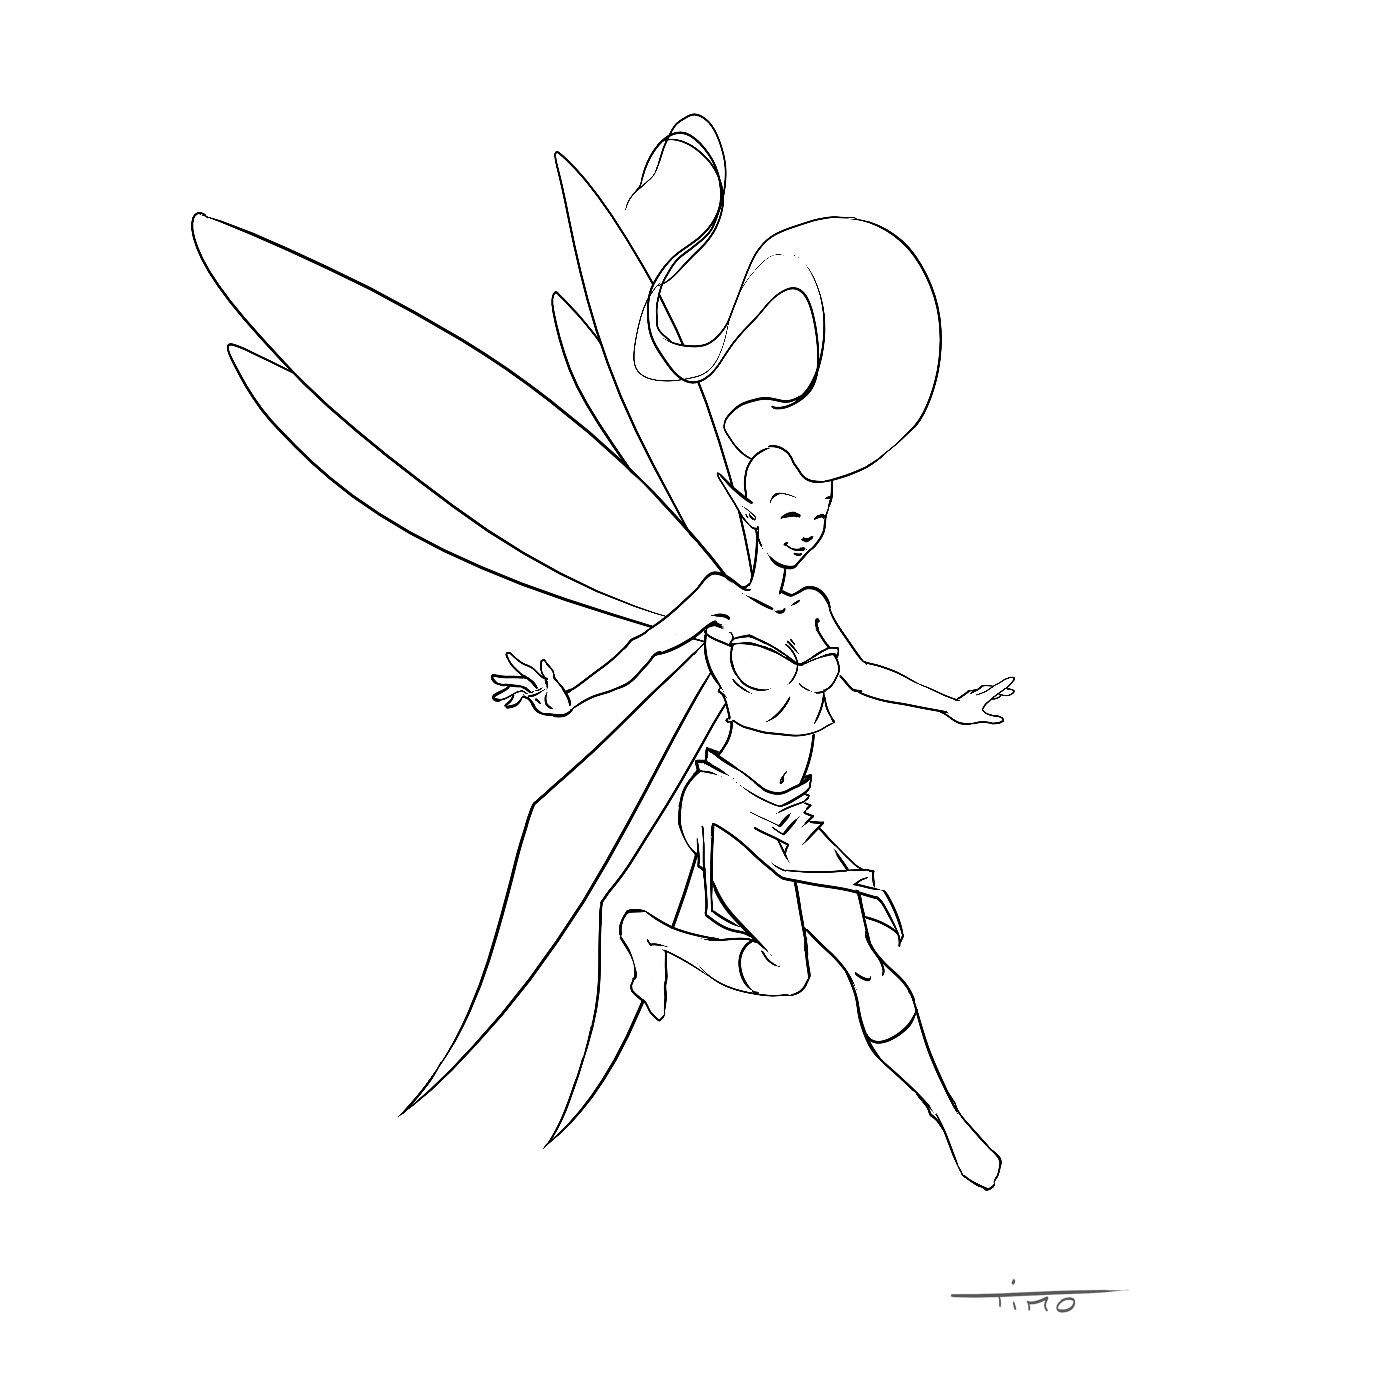
\includegraphics[scale=0.17,keepaspectratio=true]{./SeaFaery.png}
\end{center}

\chapterwithauthor{David Narváez}{A Learning Paradise}

\authorbio{David Narváez is a PhD student in Computer Science at RIT in Rochester, NY,
USA. Originally from Panama, he is the current maintainer of Kig, an application
for interactive geometry that is part of the KDE Education Project.}

\noindent{}I joined the KDE community back in 2009 to fix a couple of bugs and
never left. I was one to scratch my own itch in any application I
would use frequently: from Kig, which was my main interest, to KDevelop
which I used to work on Kig, to Plasma because I was using it to
manage my desktop environment. KDE was certainly not the only
FOSS community I contributed code to, but no other community was as
enticing as KDE. At the beginning, I could not really point the
finger at what the reason for this was.

At the same time I was learning the trade as a professional software
engineer (which, in my culture is nothing but a name for a glorified
computer programmer) back in Panama, my home country. At the peak of
my contributions to KDE, I had a full time job as a software engineer,
coding several hours a day, only to come home and code several more
hours working on KDE-related stuff. Many would say I spent my entire
day coding, but for me these were two completely different activities.

I eventually realized that the differentiating factor was
learning. KDE was much more than a developer community for me: it was
a learning environment. My daytime job, on the other hand, did not
foster innovation and learning. This was not a problem particular to
my employer at the time, but a more general issue about the culture
among software developers in my home country. While I understand not
everybody is as excited about learning as I am, I can objectively
argue that KDE, as a learning community, prepared me better for a
global market and gave me a better chance at several other
opportunities that came by later in life. Here I describe some of the
core values I found in KDE that I could not have found inside the
software developer market in my home country:

\begin{itemize}
\item In KDE we have a horizontal structure promoting code review,
  open design discussions, collaborative coding, etc. In contrast, my
  daytime job at the time had a vertical structure where fixing bugs
  in somebody else's code was considered an offense, and trying new
  technologies was never an option during design discussions.
\item Proposing the adoption of new ideas and paradigms in my
  workplace would almost always meet the mantra of "we have always
  done it this way". In contrast, I joined the KDE community as a
  developer just a couple of years after KDE adopted a whole new
  approach to desktop environments through KDE 4.
\item KDE is, by definition, a global community. As such, you will
  always deal with not only different time zones, but also different
  cultures. I vividly remember waking up at 5 am in the morning to
  read code reviews from people at 7 hours difference\todo{native speaker check}, and work on
  their feedback before leaving to work. Right around those years, the
  software development market in my home country was starting to
  globalize, and as a consequence, people started thinking about
  different time zones. When it was my turn to deal with these issues,
  it felt like home because of my KDE experience.
\item From the merely technical point of view, the various software
  architectures used across KDE projects made it possible for me to
  explore paradigms and designs that were not popular inside the
  market in Panama. My exposure to these ideas turned some of the more
  challenging tasks of my day job into straightforward adaptations of
  problems that had already been solved inside the KDE community.
\end{itemize}

I am convinced it is because of all these values we have forged
as a community inside KDE that I was able to pursue many opportunities
that would have been way out of my reach had I been equipped only with the
knowledge I could acquire in the local market. But Panama is not the
only country in the world where the digital divide is keeping
developers with great potential from acquiring all the knowledge they
need to be competitive in the global market. In fact, most of the
skills and experience that are highly valued in the IT market (think
of fluent English, or early exposure to computers) are native to a
small fraction of the planet which we usually refer to as the first
world. In the age of information, communities like KDE play the role
of forges of global talent that will enable important changes in our
digital lives. And although my personal journey in KDE has improved my
IT skills, the global talent we attract as a community does not
necessarily need to be programmers: some of our most active
contributors work on designs, translations, technical writing and even
marketing; all of which are areas with their own global markets and
needs. What is in it for all of us, is that our participation in the
community also brings along experiences that are stepping stones in
our paths to achieve personal goals.

Today, I have moved away from the industry and into research, doing
doctoral studies. This move has meant leaving my home country,
adapting to new places and having less time to contribute code to Free
Software in general. Yet, KDE is still an important part of what I do
and, as such, I care about its future. Since I consider the KDE
community an enabler of opportunities, I see our products as means to
a greater goal that is helping the world through innovation. This
point of view is what drives me every time I contribute to KDE,
because it is as exciting to think about where I can take KDE as it is
to think about where KDE can take us. Thus, it is my first and
foremost priority, looking into the future, to preserve this nature of
our community. I believe this, and not the technology we produce, is
the key to staying relevant the next 20 years. In this context, outreach
and mentoring naturally translates to more opportunities as more
people get involved, and I cannot think of a better excuse to strive
for world domination :)

\chapterwithauthor{Kévin Ottens}{Meet the Gearheads}

\authorbio{Kévin Ottens has more than 12 years experience working with Qt. He is
also a long term contributor of the KDE community where he focused for a long
while on libraries API design and architecture. Graduating in 2007, he has a PhD
in artificial intelligence. In 2012, he participated in the creation of the KDE
Manifesto. Nowadays he spends time rethinking his job via a strong interest in
Software Craftsmanship. Kévin's job at KDAB leads him to contribute to Qt~3D but
also includes giving trainings and the responsibility of community liaison with
KDE. He still lives in Toulouse where he serves as part time teacher in his
former university.}

\section*{Introduction}
As I am writing those lines (in 2016), I am 36 years old. I have been KDE
products user of since 1997, it has been 19 years, almost half of my life, almost
as long as the community existence. I finally decided to get involved with KDE
as a contributor in 2003, almost a third of my life. Also, I intend to stay
involved somehow. If everything goes well (for the community and also for me),
at one point my life without KDE will be anecdotical compared to my life with
it.

Why am I telling you all this you may ask? Well, I just want you, dear readers,
to realize that it has been an awfully long time! And now you might just wonder
\emph{``Why? Oh Why? Someone in his right mind would do something like this?
Why spend your youth working on something which won't make you rich or famous?
Why even contemplating doing that while being older? Don't you have a life?''} \\

This is a lot of valid questions and I'll try to answer it simply with this:
\emph{you can't and shouldn't get rid of your family}. That might still sound
mysterious, so let's expand on this idea.

\section*{How It All Started}
For as long as I remember, I wanted to do something related to computers and
later I decided I'd at least try myself at AI topics because of William Gibson's
Neuromancer. In 1996, I bumped into my first Linux distribution (a Slackware
spin) and got hooked on the Free Software culture as a result, it was only a
matter of time before I ended up contributing to something. \\

I had this hunch that I would likely contribute to something I use... so I
tried to use mostly Free Software which source code I felt comfortable with.
Yes, it means I chose by looking at the code of the software I evaluated, not
by its looks or by how many features it stacked (those criteria came only
distant second). Needless to say that quite a lot of the software of the time
wasn't really to my liking. In the end, the source code coming from KDE
impressed me most so I started to use more and more of it, waiting for an
opportunity.

Finally, I found a missing feature for my workflow in the desktop of the time
and decided to make a plugin for it. Instead of keeping it for me, I decided to
contribute it to the world and was greeted by a crazy Canadian who maintained
Kicker at the time. My plugin ended up part of the next official release. \\

That was obviously a very encouraging start. Still, this is mostly about
technical facts and some distant political vision. Nothing which could explain
being engaged for long with the same community.

\section*{``Happy Families'' Meets the Lunatics}
I started for technical reasons, but really, I stay because of the people.
When I got into KDE, it sometimes acted like a large, funny and chaotic family.
It was also quite dysfunctional at times... like most large families. I think it
still is like that. This is probably important for bonding people. Obviously,
you see quite a few stereotypes in such families. I think I witnessed quite a
few of them. \\

Indeed, while getting in the community I met plenty of characters... \\

The clever emo-goth cousin wearing only leather and weird boots. You don't
always feel comfortable with him since you're not sure how he is going to react
when you might point out something flawed he did. He also tends to express
weird offensive opinions in public just for the sake of it.

The aunt you admire hoping to be one day a bit like her. The clearly inspiring
person that takes you under her wing with great pleasure. If you pay attention
you will likely get insights from her wisdom. You might not understand it at
the time and might realize it only later.

The uncle you like to tag along with because you know the time spent will be
fun and crazy. He gets you to places you'd never go to (karaoke bars anyone?)
and do crazy things, like talking to drunken strangers in a foreign town.

The grandpa who is a great story teller. You always love spending time with him
late during family reunions. When the great noisy time is gone, he is still
around gently counting real or made up stories.

The grandma who had several lives. Clearly you can get wisdom from her
experiences. That said, you also get the feeling that sometimes she is getting
overly conservative and over-protective. \\

As a long timer, I also ended up in the oldies group, which gives you a whole
new perspective... \\

Two sisters you appreciated, stopped talking to each other because of some feud.
There might have been something valid years ago. Unfortunately, years after
instead of being put to rest, one is estranged and some relationships in the
family are still tainted by it.

The little cousin with attention deficit who brings plenty of new activity
ideas for the whole family... but unfortunately he rarely delivers completely
and someone else picks up to complete the vision.

The little brother still trying to find his place in the family. He is still
feeling insecure but in time he'll grab the torch and move the family forward
together with his whole generation. It is a privilege to see him grow. \\

Of course, there are many more such characters in our community and that is what
makes it interesting, unfortunately I can't list them all here. My hope is that
by pointing a few out bluntly it'll help members to reflect on their peers and
try to improve how the family works so that it is rarely dysfunctional.

\section*{Conclusion}
Yes, I do have a life... and it involves all the KDE family characters in some
twisted way. This is not the kind of thing you really think about as a child, you
don't envision something quite like it. But it happens. Most of us start because
of some itch to scratch or technical curiosity, this is hardly a rational choice
in the first place. \\

Similarly, I'll slightly change Desmond Tutu's words: ``You don’t choose your
family. They are [the Universe] gift to you, as you are to them''. \\

Clearly, KDE has been a gift to me, a second family. This is why, just like for
my first family, I try to be available for fellow gearheads and be a gift to
them.


\chapterwithauthor{Valorie Zimmerman}{Why I chose KDE, and why KDE is family} 

\authorbio{Valorie Zimmerman is \todo{add bio}}

\noindent{}Around 2001, my son showed me two desktops, and asked me to choose which one I wanted on my new install of Mandrake. I chose blue, the pretty one, and so began my KDE journey. Back then, I understood very little besides that I found KDE software to be not just more beautiful, but also usable and configurable. 

Before contributing to KDE, life was busy with kids and work. Fortunately a friend introduced me to Linuxchix, so a friendly group who helped out newcomers welcomed me in. I met people who contributed all up and down the stack, including Windows users like me who were considering a move to Linux. So Linuxchix was my way in to KDE and Kubuntu.

Back in those KDE3 days, KDE was still a bit controversial in FOSS circles. Qt licensing concerned some people and the whole KDE vs. GNOME 

If any group wants to grow, it must have ways in. For KDE, I found IRC and mail lists first. Many women on the Internet find the hostility and bad behavior discouraging enough to never find their way in. Fortunately I had the Linuxchix at my back, and found KDE mostly welcoming. When I spokie up to volunteer, people enthusiastically replied, and gave me good suggestions about how to start. I found that very project needs better documentation! Growing groups will do everything they can to help you get started. I began in Amarok, which was such fun. After looking through old docs, and considering the options, we decided to do the Amarok Handbook on Userbase. Not realizing that this was somewhat pioneering, we just plowed ahead, and used the old docs to make new pages in Userbase. It was great to work with Amarok developers, KDE doc folks, along with the wonderful web team that has been keeping the wikis so useful to us. 

A word on volunteering. Early in my "KDE career" I volunteered for the Community Working Group. Little did I know what I was getting into! That said, tackling the difficult issues between developers has been rewarding, because peace is usually the result. At the very worst, we know we tried our best to create a good situation out of a bad one. So blithely heading towards the cliff-edge like The Fool on the Tarot card, has been a good move. Getting to know people deeply is wonderful. Being a part of the CWG team has continually reminded me why KDE is family. Learning how to listen better, how to "fight fair", how to recognize issues as they are forming, and then helping them go in good directions, have made all of us involved better humans. I salute all the past, present and future members of the team, and peace-makers all around the world.

When the first Google Code-In was announced, those of us on the Amrarok Handbook project immediately thought about all those unwritten pages, and began creating tasks for students; one task equaling one page. What a fantastic experience! It was wonderful to interact with those kids (ages 12-18) and help them help us. Once involved in GCi, which was intense, exciting and productive, I was hooked on student programs in KDE. Looking back at the students who have worked with us over the years, one can see that student programs creates the future of KDE. Our students begin working with mentors and teams, and our goal is always to welcome them into the family of KDE. Many of our most successful initiatives are now being run by former students, and many of our most effective mentors were once students themselves. Working with the Student Programs team has been so satisfying.

One of the things I love best about KDE is that while we do the inward-looking work, such as improving our processes, governance, and social relationships, we are generally outward looking. We don't simply make software that pleases us, but follow our ideals when working. I see developers write tests for their software even while complaining about how boring it is, simply because they value quality. I see people step up to write Dot stories, release announcements and blog posts even when they dislike writing, because they want to share our work with the world. People comb the code for spelling errors and other small issues, and quietly fix them. Document writers do the same thing with the documentation -- fix errors, test the texts to be sure they are up-to-date, contribute new screenshots -- all quietly and often un-acknowledged. Our Visual Design Group created itself out of nothing, and quietly steps in to help application teams, Plasma developers, and web-workers. The Sysadmin team is tireless! They keep our infrastructure up, humming along happily, and most important: securely. They create new structures to help out the developers, and improve old ones. We have folks working upstream in Qt, making, for instance, accessibility Just Work for everyone. Many faithful KDE members also work "upstream" and "downstream" however you define that. Our distributions are richer and healthier with KDE involvement, along with many other FOSS projects in the ecosystem that surrounds and supports us in turn.

All of this work affects all of us in KDE every day, but we may not notice it unless there is a problem. The focus on freedom and quality is now even moving onto platforms beyond Linux and BSD in a major way. Even folks who don't use Android, Mac or Windows have generously contributed to support developers making our applications usable to an even wider population. This generous spirit and welcoming attitude is what has kept me, a grandma, involved in creating KDE as long as I am able.
\chapterwithauthor{Nuno Pinheiro}{The transient nature of design}

\authorbio{Nuno Pinheiro is a Portuguese graphic designer and illustrator. He specializes in iconography, themes and user interface design. Nuno's works include general illustrations, UI design, web design, corporate design as well as other works in creative areas. Known for his work in the Oxygen Project where he is the current coordinator of a design platform with 2000+ icons, wallpapers, sound effects and window styles. His computer art is used on KDE computer platforms worldwide.
Over the last years he engaged in coding with QML creating fine tuned experiences for users and became interested in the Developer/Designer Interface.
He works as a UX/UI designer, consultant and trainer at KDAB.}

\section*{The Tempos of Oxygen}
Design in open source is special. At least to me it is, and has always been, and the reason for that is simple: the relative ephemerality of it, so unlike other open source projects where the beginning is well defined but the end is something to be avoided. In design and especially in this post-modern ever-recursive design landscape the end is as present as its beginning, and so it must be fully embraced.

So... What is the point of it? I mean if it is done to have an end what does it achieve? This creates a problem that I'm sure every design related open source project has debated with itself.

For Oxygen and me personally it was solved with the assumption of three time periods: a future, present and past. That looking back has now been reverted.

\section*{Its Past was its Future}
So what drove me to design and open source? 
I guess this is where, for me, design shares more with common “traditional open source projects”: an itch to scratch, or more specifically a couple of emoticons in an instant messaging app I used in my favorite desktop at the time (KDE 3.X). So I made a couple of icons (really low quality) but was encouraged by the wonderful community to keep working on it and so I did. And as a result of my continued engagement with the community, I was invited to be a part of this new project – Oxygen. In its infancy it was a Future, it was everything, and anything, the solution to all problems. It was also a repository of all my uncertainties and doubts (all founded, I might add), but it was a fantastic time, a time to get to know what you are and how you express it, a time to realize that working within a group of people is far more challenging but also far more rewarding than all by yourself. A time to make mistakes, a time to correct those mistakes and a time to realize the extension of your errors would mean, you would need to start all over.
In the end what comes out is Oxygen, a child of its time, a son of Everaldo Coelho, Crystal Icon set of Nuvola by dear friend and Oxygen colleague David Vignoni. It was an icon set and it was amazing.
The future offspring of some superb parents - and trust me we stood on the shoulders of giants - for its time Oxygen's parents were, in many ways, ground breaking feats of computer design not just in open source but in computer design, rivaling with the best of the best in the industry.

This realization, personally, made me become fully aware of the absolute certainty of Oxygen's own future and goals: Oxygen should strive to be as successful as its parents, and most importantly, set new future children\todo{native speaker check}.

So in my mind Oxygen was something for the KDE 4.X series. Beyond that something new would have to take its place.  


\section*{Its Present, where Past and Future face each-other}
So you have this group of people, that are making an icon set, and in the constant struggle between past and future, you keep on creating new futures in order to move on, so you get more people involved in the project and you add new futures, new projects, new ideas, and the icon theme becomes so much more. This is the explosion phase. An icon theme becomes a Qt theme, a sound theme, a design platform – 1000 different things!
Personally, this is the time that made me a designer. Never underestimate the power of trial and error. A lot of practice does not make perfect but it sure helps you to get better.
The icon set suffered many mutations as it defined itself thought time, the Qt theme, Plasma themes, Oxygen and Air, the cursor theme, the sound theme, the multiple websites, the countless posters, banners, mugs, pins, meetings, talks, etc, etc,... amounted to gargantuan amounts of work. 
Make no mistake it was an absurd and gigantic effort, it was incredibly fun and in a way it set, what I personally consider, Oxygen biggest achievement.
Before Oxygen, design projects in the open source world tended to vary from uncoordinated projects that lived in the same space, to vaguely related projects where different groups would coordinate design visions so that desktops would have some sort of coherent visual language, for example: the good efforts from our friends at the GNOME Desktop, and the multitude of projects it created but that shared an obvious vision and language.
Still Oxygen was different now. It was so much more than just an icon theme. It was anything you would see in your desktop and more. We went to the extreme of making Gtk themes so that the KDE experience would be even more consistent for the users. Hat tip to a great Oxygen guy, Hugo Pereira for his outstanding work in this area.
Oxygen might not have been the best icon set of all times (it was good enough in my opinion but not as ground breaking as its parents were) but the scope of design efforts was unprecedented in the open source world. 
So to me, Oxygen's development period, “present”,  was a success - maybe not from the pure creativity design language point of view (I'm not even sure if I'm unbiased to say anything truly fair about its merits in that regard), but from what it set as the goal post of what a design project in open source should be. I believe it did reach its goal by setting a new bar level\todo{native speaker check} of what to expect from open source design projects.

\section*{Its Future or the starting of a new Past}
Some years ago Qt released Qt 5.0 and, as anyone that knows something about KDE knows, that means big changes are coming. Add to that the mobile explosion, the touch explosion, the QML language and Qt Quick revolutionizing things and the relative importance of design in computer user interfaces.
This meant that visual languages and user expectations were changing. Also my expiration date on Oxygen was reaching its due date with series 5.X's on the horizon.

A perspective of making themes, even coordinated ones were not enough to create meaningful competitive user experiences.        
Oxygen failed to be that. As a result of the way it evolved and what it consisted of in its inception it was hard to be anything else than what it was. This new method of doing things in some ways would defeat the propose of consistent theming, just like architecture and urbanism rules are different things, so are consistent theming and perfectly tailored user experiences different and not fully compatible concepts.    
So at the end of the Oxygen period, user experience and user interface design was reaching an inflection point. Gone were the days were graphical designers challenged their own illustration skills in a perpetual "I can draw my candy more naturalisticly silly than yours".
We had reached the saturation point of the silliness in graphic representations of every day objects as user interface elements. Now back then people needed to find a culprit for it all, a quintessential word that in itself represented all evil. Cue in "skeuomorphism", a word used in traditional design to imply a faux representation of a material. In this word we collectively found the "wrong" to be corrected. We had our culprit.
Well all of this to me, back then, sounded a bit like a personal attack. I mean, gradients and shadows was all I did, and just because some were abusing it I had to pay for it? Yeap I did!

Plus Oxygen was starting to look old, in my eyes, and I knew it was time for something new, something fresh. 
The true testament to Oxygen's relevance was about to be put to a test. Would it be replaced, would some breeze of freshness be able to correct all wrongs in Oxygen?
To be absolutely honest, I was worried. For some time it seemed no-one would pick up the work, and from a personal point of view I felt I needed to take some timeout to reinvent myself, so I should not be leading a post-Oxygen design language.

But the magic of open source did offer us, collectively, a new set of fresh people in the form of the KDE Visual Design Group, and with that Breeze, a new past of something new that was its future.

Oxygen will still live on the 5.X's series of Plasma/KDE desktops and I will keep on maintaining it, but now there is a new being that Oxygen failed to be. And it is great.
This was achieved by far more than just me, it was/is a wonderful group of people - some of them I mention above, and trying to mention them all is impossible; but being incredibly unfair to all of the ones I will not mention, a word to Riccardo, Marco, Sho, Bettio, Ken, and all of the users: an enormous Thank You. 

\section*{Conclusion}
So when starting this article the point I wanted to make was the transient nature of design in open source projects. Its announced death at inception time is not something to be taken as a bad thing. It is a natural event that should be embraced from the beginning, the fact that it will have three tempos and that they will cross within themselves is a natural thing, on its way to reach conclusion, that its mortality is nothing but a step into a new birth.
I wanted to say that I knew this from the beginning and that it made me happy that everything went as planned. It did and it is true that I am sincerely happy about the little apparent loop of creation, the cheating of death by continuity, a glimpse of immortality, via the ever chaotic butterfly effect. And this would make a nice enough conclusion advising you, the designers, to embrace open source projects with that in mind.

But... Thinking a bit more about it, I have to be more honest, I have to look into what drove me, what motivated me. I mean having a plan and executing it when you previously define that very plan according to a pattern that you see as the only possible best outcome may feel a bit mechanical, and it was nothing like that.

... and then I remember, people used to ask me all the time “how come you do it?” and I would answer “because it's fun”, this simple answer was my real truth, maybe this is all it boils down to, that terrible cliché. It's not the destination it's the journey, the journey is what makes life and at the end of the day life is only true if you do, see, feel, create, quit, restart, win, lose, and love, yes love. Love what you do! I Loved doing Oxygen. I love doing open source design.

\chapterwithauthor{Volker Krause}{Twenty Years of Email}

\authorbio{Volker Krause joined KDE in 2002, and primarily contributed to KDE's email and personal information management infrastructure and applications. He works as a software engineer, consultant and trainer at KDAB.}

\noindent{}On October 14, 1996 Matthias Ettrich started KDE, with an RFC822 message, the same message format still in use today two decades later, with just minor fixes and extensions for supporting non-ASCII text. We all know this as email.

Shortly after, still in 1996, KDE's own email client, KMail, was started. While it mutated heavily several times in its almost twenty years of history, you can still find traces of its founders in the code today.

Email has always been an essential companion of KDE. A lot has changed though, and will continue to change. It is interesting to look at the developments and challenges in this way, as these are also reflected in many other areas of KDE, and beyond.

\section*{Enabling Access}

Back when KMail was started, the prevalent way of using email was downloading and storing it locally on a single personal computer, with ISPs or universities providing POP3 accounts that buffered incoming emails until the user had a chance to fetch them. With email becoming popular and important on a larger scale, various companies tried to push their proprietary variants, such as Lotus Notes and Microsoft Exchange.

Therefore the first challenge was to provide free access to email, both free of cost and with the freedoms guaranteed by Free Software. This might seem odd from a present point of view, where we are used to finding Free Software applications for pretty much any use case.

In the first years of KDE, Free Software as such was not yet universally accepted. On the contrary, it had to face massive opposition, in particular from Microsoft. It took years to prove that Free Software was a development model that could provide high quality and innovative applications, something that is hardly questioned anymore by now. Even Microsoft is contributing actively to Free Software today.

KMail, together with many many other Free Software applications, proved the opponents of the GPL wrong, having become a competitive product, with some of its innovations such as the missing attachment warning having found their way into many other email clients. And it has found a balance between purism regarding open standards and pragmatism when it comes to compatibility with proprietary applications, still an ongoing discussion in the Free Software world.

In order to enable free access to your data, free applications are essential. As the world changes however, this is challenged over and over again, and free applications are not the only piece in the puzzle any more.

\section*{Clouds}

As computing equipment, and email with it, became more and more ubiquitous, a new challenge arose at the beginning of the century. With the availability of laptops, and later smartphones, email needed to be available on multiple devices simultaneously; the old download model did not work anymore.

With the widespread availability of permanent internet connectivity in the wake of the dot-com boom, the solution turned out to be server-side storage and online access, an approach that years later became associated with the term “cloud”.

IMAP, the protocol for server-side email storage and access was standardized, and KMail received support for it. While solving the problem in theory, the limited availability of email providers offering affordable IMAP hosting at the time did not really help though.

Instead, advertisement-based webmail providers started to appear and became popular, offering cost-free email hosting with access from a browser, and a few megabytes of storage space. That entire market got swept away with the appearance of Gmail in 2004 though, which offered an (at the time) audacious one gigabyte of storage space, and a stream of innovations in the user interface. Gmail has since become the de-facto standard for consumer email.

The implications of this were not immediately recognized by everyone, and the inside perspective tends to be skewed. We understand the risks and implications of the cloud approach (“there is no cloud, just other people's computers”), and we have access to alternatives, but that is not what the average user sees when looking at Gmail. It is a solution to a very real and pressing problem, and even seemingly free of cost.

KMail, of course, has dedicated support for Gmail and its various non-standard extensions nowadays. But regarding having control over your own data, is that really the way we envision our communication infrastructure?

How and where data is stored and how it is accessed have become just as important as having a free application to access it, and this is more than providing a Free Software server implementation. We also need to offer solutions for secure and reliable hosting and deployment. “Just run your own email infrastructure” is not a viable solution for most users. Finding convincing and practical answers to this will be an important challenge for the Free Software community in the coming years, KDE included.

\section*{Small Screens}

In 2007 the iPhone started the age of the smartphone. A year later, Android followed. By 2012 a billion devices had been sold, making a small touch screen with barely more than a ten centimeter diagonal the world's primary communication interface.

First attempts to give KMail a smartphone-compatible interface happened in 2010, with limited success. The way we organize and use email is inherently tree-based. Folders, message threads and inline conversations can all get deeply nested. Tree-based interfaces however only work poorly on small screens, either being very cumbersome to use or imposing severe restrictions on the nesting depth.

Not only KMail was affected by this challenge though. This also contributed to the rise of a new style of communication approach\todo{native speaker check}: the messenger apps. By linearizing conversations, they avoid the user interface challenges email poses on small screens, quickly gaining hundreds of millions of users.

Unlike email however, the messengers, no matter if using proprietary or open source clients, are not using standardized and interoperable protocols, turning them into communication islands relying on vendor-hosted server infrastructure.

Gmail and proprietary messengers are challenging conventional email clients, in particular in the consumer space. Even heavyweights like Thunderbird struggle with this. Solutions that allow you to regain control over your communication data, without losing the convenience and functionality proprietary solutions provide right now, have yet to be found.

\section*{Silos}

The smartphone platforms also made application bundles a widely-used technology, to support their application stores and increase security on the devices. Application bundles since then have also become relevant on all other major platforms.

Isolation from broken or malicious applications and straightforward deployment and cleanup make application bundles a very attractive choice.

On the other hand, application bundles lead to the creation of silos. Data and functionality is only available to a single application, and the rest of the workspace cannot benefit from it.

With KDE being both an application vendor and a platform vendor in this model, KMail is faced with with a dilemma. In order to be easy to deploy on the most widely-used platforms (Windows, Android) an application architecture that allows the creation of an application bundle would be needed. On the Plasma workspace however, deep integration would be desirable, providing access to email communication for the entire platform.

KMail has chosen to go “all in” on the platform integration side, with a multi-process architecture enabling data sharing and non-exclusive data access. This is a prerequisite to offering a free and privacy-honoring answer to the personal digital assistants for example.

Other KDE applications are focusing on application bundle compatibility instead. There is no right or wrong here, but finding a way to serve both scenarios will be a major technical challenge for many KDE libraries and applications going forward.

\section*{Privacy and Freedom}

Providing secure communication can be traced back to the early days of KMail. Support for PGP encryption was added in November 1997, and support for transport encryption followed soon after. Growing interest in security, also in the form of public funding, resulted in the joint Gpg4Win project together with the GnuPG community, with KDE providing the Kleopatra certificate manager.

In May 2013 Edward Snowden gave the world a glimpse of the extent of global mass surveillance. What were once considered naive assumptions suddenly looked naive\todo{logic}, and unless you took measures to protect it, privacy turned out to be hardly more than an illusion.

Not only is all your communication intercepted and recorded, it is also automatically analyzed by machine learning algorithms that decide what is “normal” and what is suspicious. You lose your freedom to be different, and uncontrollable machines decide the consequences of that. It has become very apparent that privacy is an essential prerequisite for freedom.

Free Software is well positioned to ensure privacy when it comes to your digital footprints. Free Software is probably the only way to ensure that. And without conflicting commercial interest in KDE getting in the way, our users are not our product, and we can truly follow the “privacy by default” maxim.

As news about the extent of the mass surveillance spread, demand for Gpg4Win tripled, with monthly downloads crossing the 100,000 mark. KMail also saw a renewed interest in improving encryption features, in particular by making them easier to use. “Privacy by default” also means the software needs to do everything it can to ensure privacy if the user does not understand the intricate details of public key encryption and certificate trust chains.

Today KDE technology is helping millions of users to protect the integrity and privacy of their email content. There is still more to do though. Content encryption is only addressing part of the issue, and protecting metadata of email communication is an equally important and still unsolved problem.

\section*{Conclusion}

Matthias got what he had asked for, and so much more. What KDE in particular and Free Software in general achieved in the last two decades is beyond what would have been imaginable in 1996.

People have questioned the relevance of the desktop, the relevance of email or that of KMail in today's world. All this of course might or might not change in the future. That is not the most important question going forward though. It is who will have control over your data. And that is not just affecting email. What is the point of Calligra if your documents are locked in a proprietary Google or Microsoft cloud? What is the point of our scientific and educational software if you cannot afford the corresponding textbooks? What is the point of our communication software if the world uses proprietary messengers?

Obviously free applications will stay a key element for this, but we also need to look at the bigger picture and continuously reevaluate if we still provide a valid solution to whatever the original problem has evolved into by now. With ubiquitous connectivity and software so deeply embedded into every aspect of our lives, we cannot look at applications on their own anymore. We need to look for solutions for today and tomorrow's use cases that allow you to retain and regain control of your data, striving for a world in which everyone has control over their digital life and enjoys freedom and privacy.

\chapter*{Closing words}

When I joined the KDE community 10 years ago I could never have imagined how much of an impact it would have on my life. I am where I am today because of the people in KDE and everything I learned from them. I am surely not the only one and I am grateful for it. In a world of rising tension between cultures, countries and people, communities like KDE transcend artificial barriers and make us understand that we are better together than we are apart, that we achieve more when we are united than when we are divided, that our shared interests are bigger than our differences.

This book can only give you a glimpse into the past 20 years of KDE. I hope we still gave you a good overview and explained why our heart is in this community.

To my fellow contributors: May you always stay innovative, smart, open-minded, inclusive, dedicated and awesome. Thank you for being a part of the journey. A lot of amazing things are still ahead of us.

To our users: The past 20 years have shown that there is a lot of technical excellence, pragmatism and will to fight for our users in this community. We will continue on this way - for you.

\begin{flushright}--- Lydia Pintscher, KDE e.V. President\end{flushright}
\begin{flushright}Berlin, Germany; 24th of July 2016\end{flushright}

\backmatter
\end{document}
